\begin{mdframed}[backgroundcolor=red!5]
This stone was partially contributed by E. van der Wiel.
\end{mdframed}

\url{https://github.com/cedrict/fieldstone/tree/master/python_codes/fieldstone_55}

\vspace{1cm}

Parameters for the setup are defined in {\sl parameters.py}.
This file is used in {\sl generate\_nodes.py} which produces the
{\sl subd.node} file which contains the coordinates of all key points 
on the boundary of the domain and along the material interfaces.
This file is then further processed by the triangle 
program\footnote{\url{https://www.cs.cmu.edu/~quake/triangle.html}}
as follows:
\begin{verbatim}
./triangle -q -a200000000 -o2 subd.node
\end{verbatim}
The '-q' option adds vertices to the mesh to
ensure that all angles are between 20 and 140 degrees. 
The '-a' makes sure that no triangle has an area larger than 
the supplied number. The '-o2' generates a mesh composed 
of second order triangles (six nodes per element, rather than three) and the
three extra nodes of an element fall at the midpoints of the three edges.
This generates two files: 'subd.1.ele' which contains the connectivity 
of all generated triangles and 'subd.1.node' which contains the coordinates
of all nodal points. 
These two files are then read in {\sl fieldstone.py} and stored in the xV, yV and iconV arrays.

Gravity is vertical and Earth-like. Free-slip boundary conditions are imposed on the top while 
the other boundaries are free (in/outflow determined freely based on the internal dynamics). 
In order to remove the horizontal null space the average horizontal velocity is set to zero. 
Crouzeix-Raviart elements are used, see Section~\ref{sec:crouzeix-raviart}.
The density of the mantle is set to zero while the subducting plate has a density $\delta\rho$. 

\begin{center}
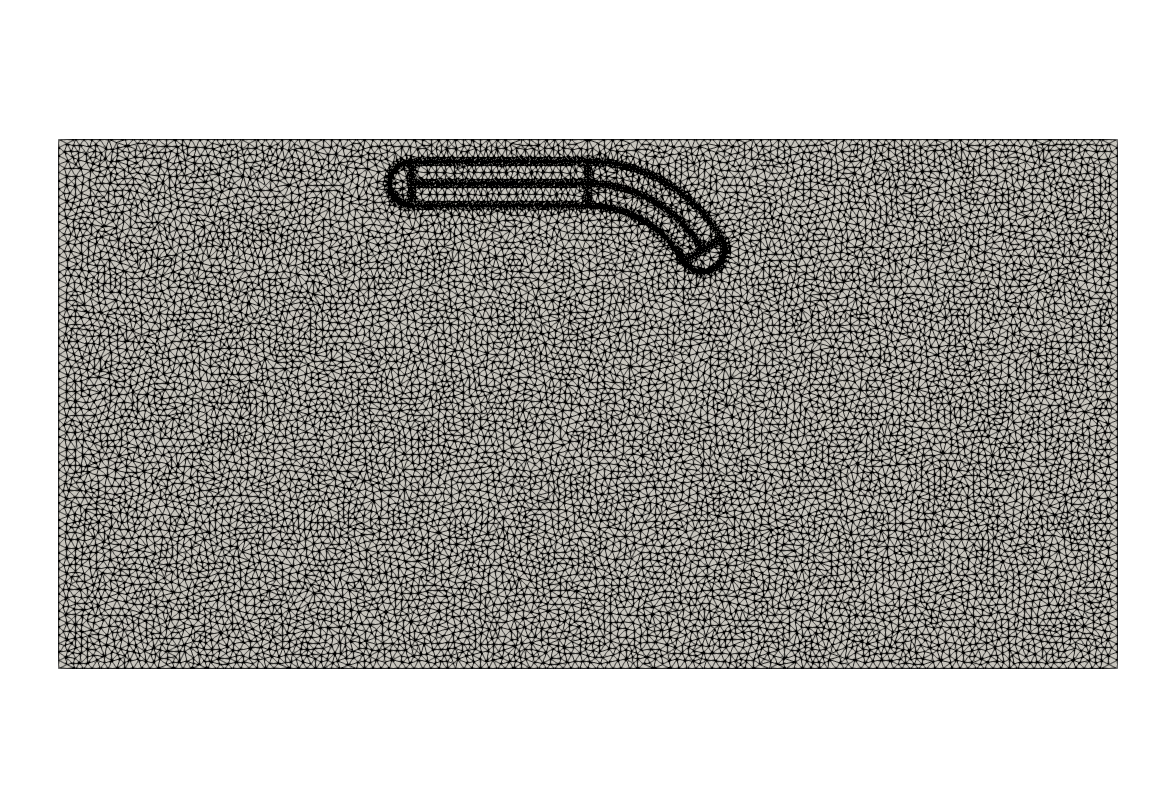
\includegraphics[width=7.5cm]{python_codes/fieldstone_55/images/mesh}
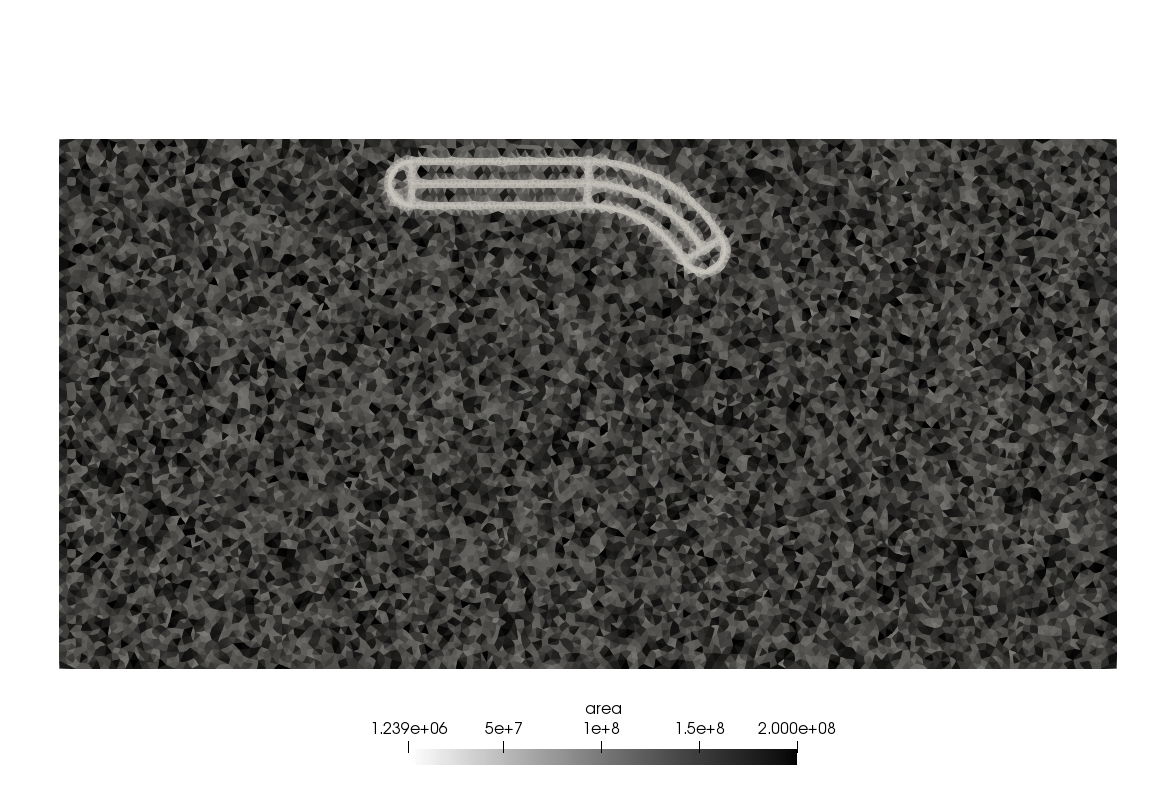
\includegraphics[width=7.5cm]{python_codes/fieldstone_55/images/area}\\
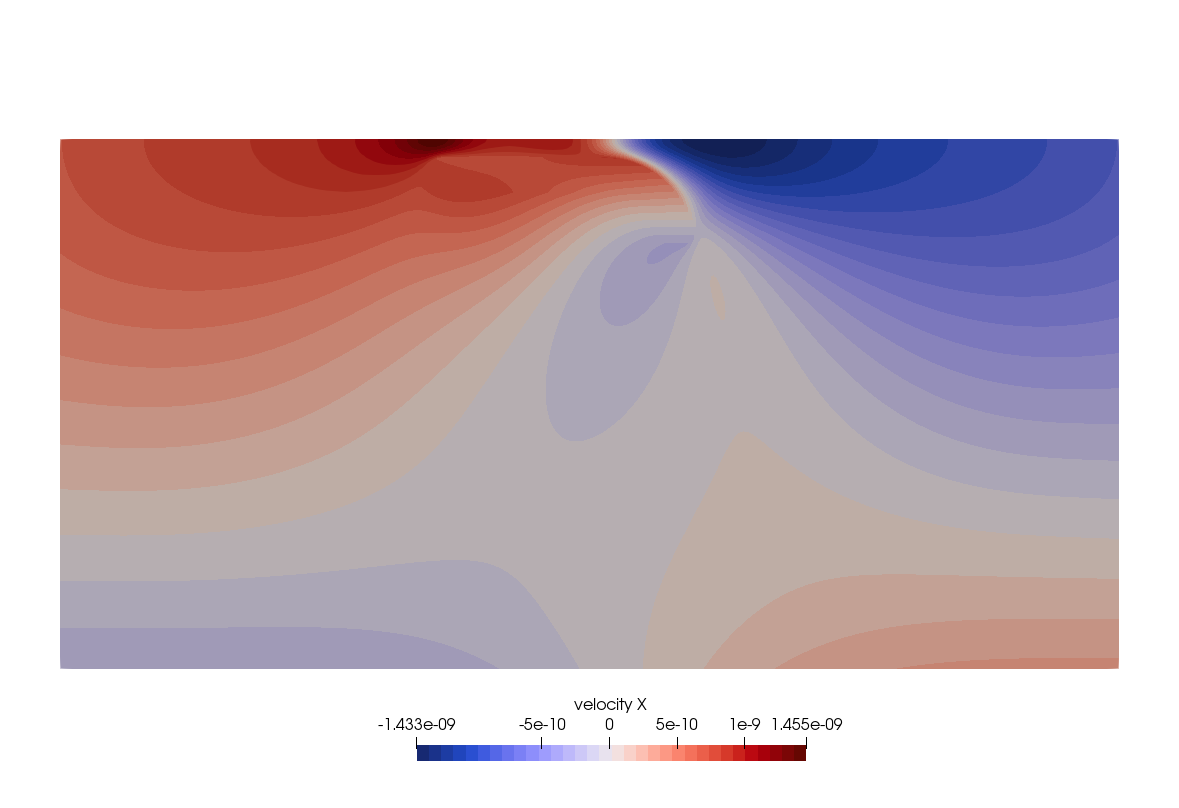
\includegraphics[width=7.5cm]{python_codes/fieldstone_55/images/u}
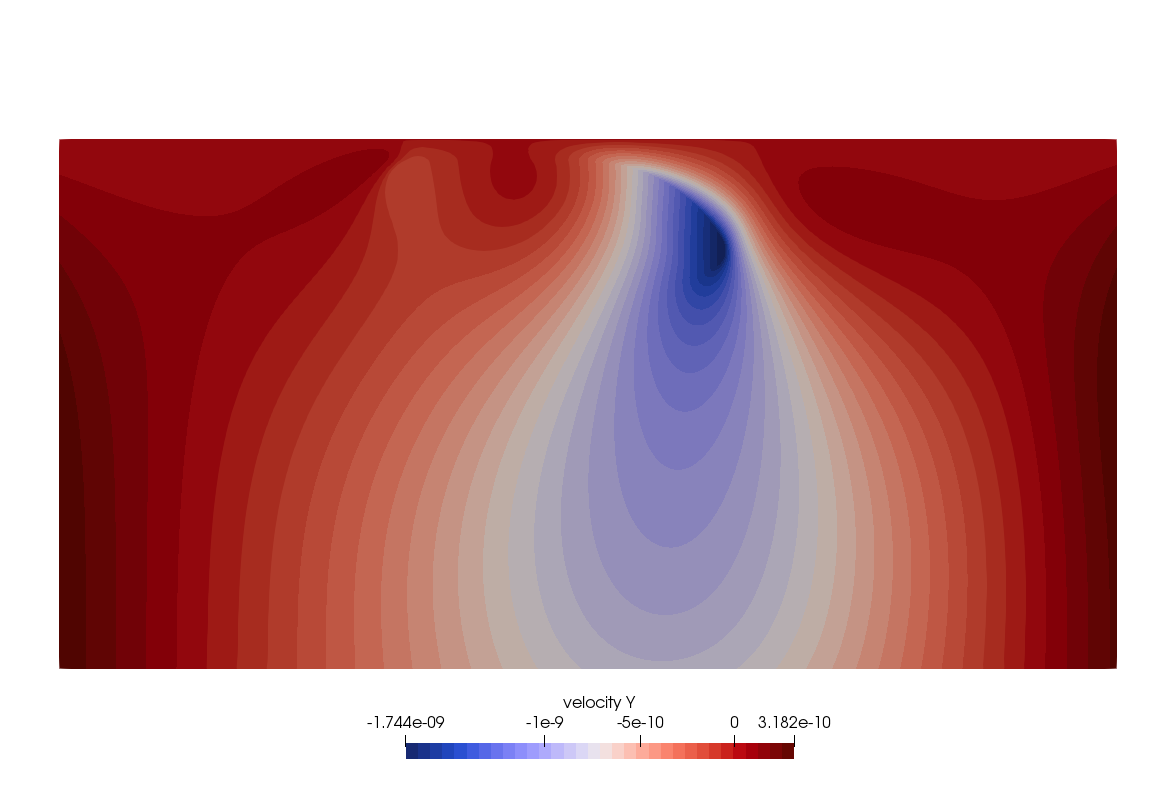
\includegraphics[width=7.5cm]{python_codes/fieldstone_55/images/v}\\
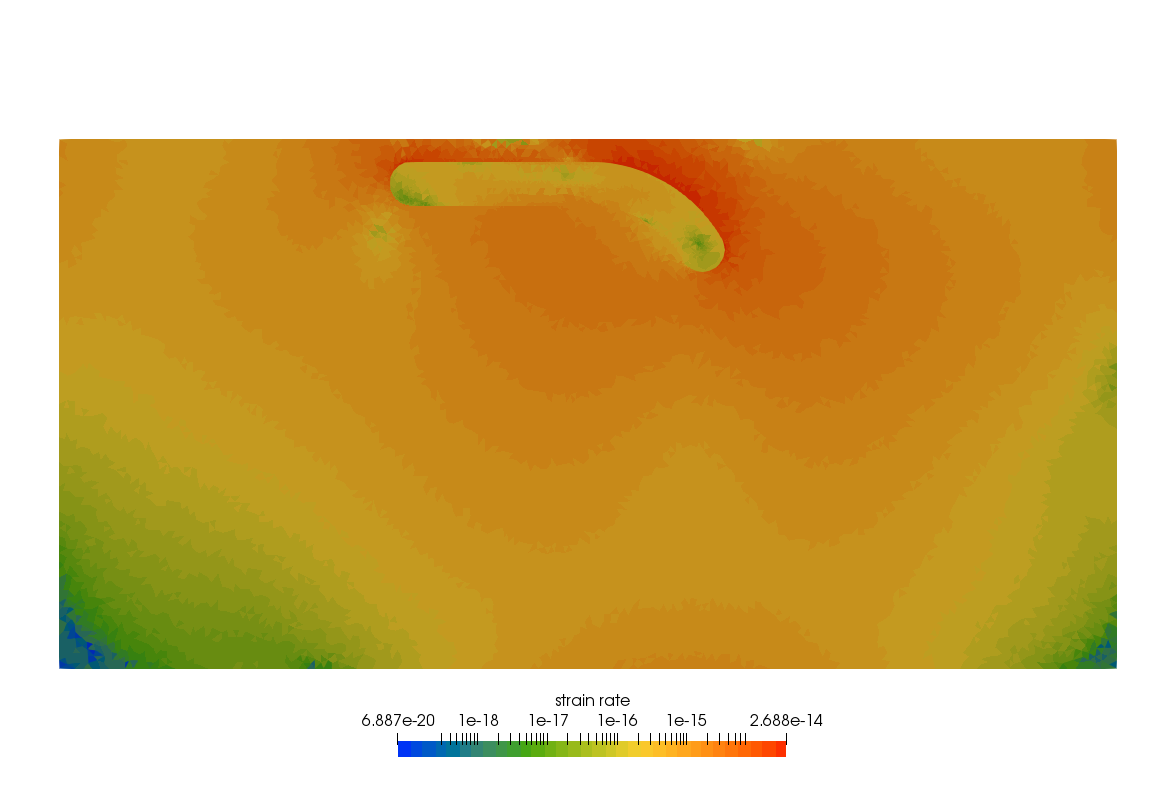
\includegraphics[width=7.5cm]{python_codes/fieldstone_55/images/sr}
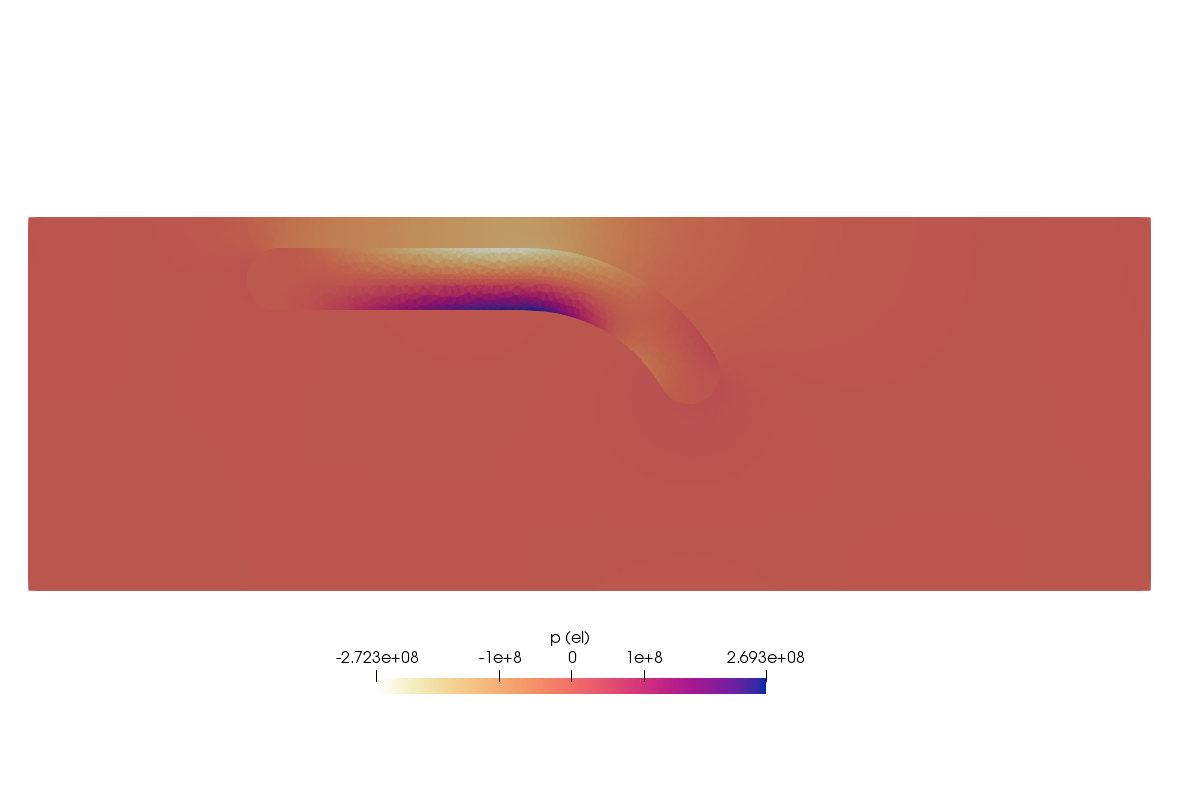
\includegraphics[width=7.5cm]{python_codes/fieldstone_55/images/press}\\
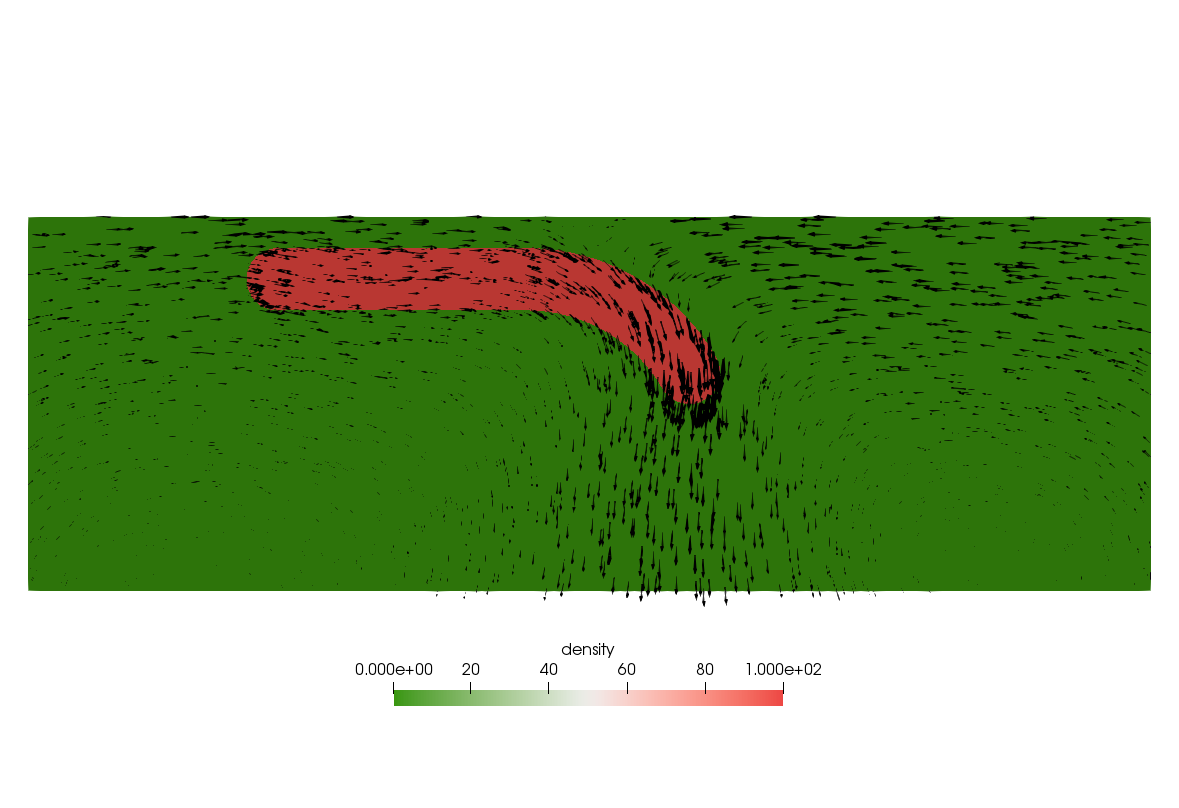
\includegraphics[width=7.5cm]{python_codes/fieldstone_55/images/rho}
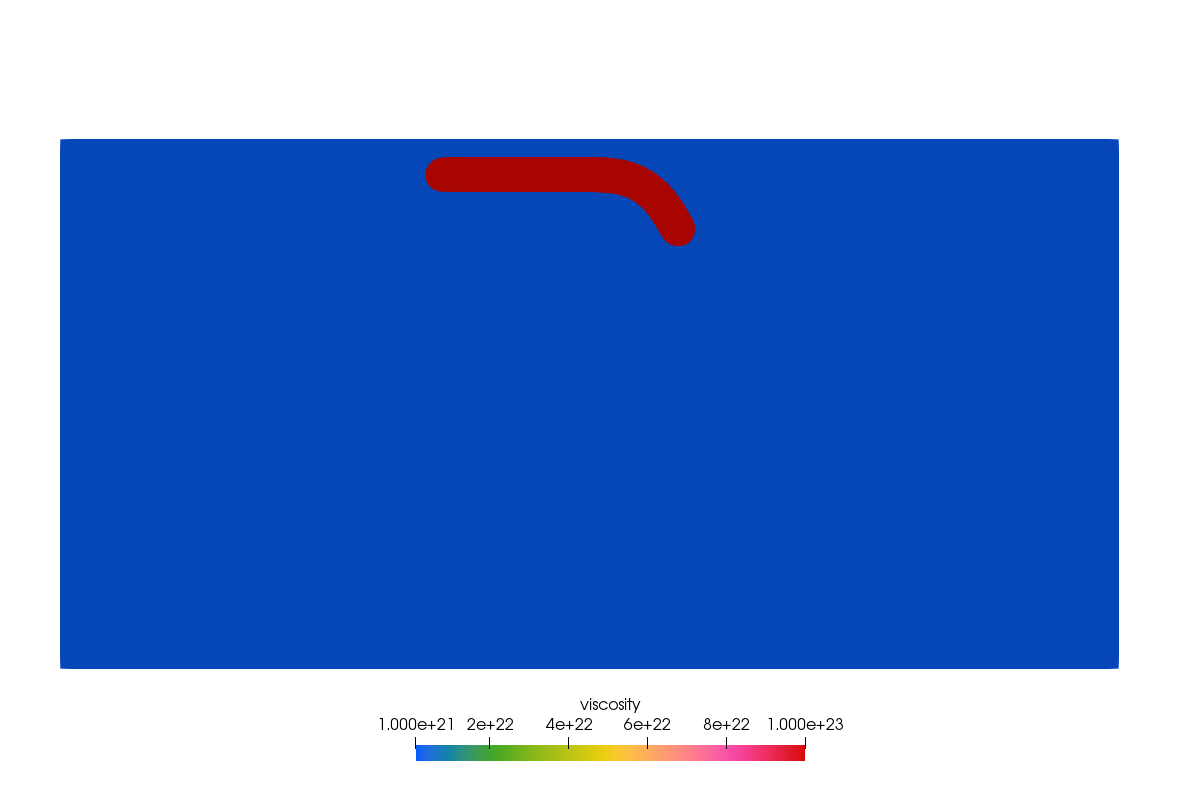
\includegraphics[width=7.5cm]{python_codes/fieldstone_55/images/eta}\\
{\captionfont Mesh composed of 31,765 triangles.
Other parameters: $\theta_0=60\degree$, $\eta_1=10^{21}$, $\gamma=100$, 
$L_x$=3000km, $L_y$=1500km, $\delta\rho=100$, $L=$400km, $h=$100km, $d=$50km. 
Note that the bottom boundary is open.}
\end{center}

%\begin{center}
%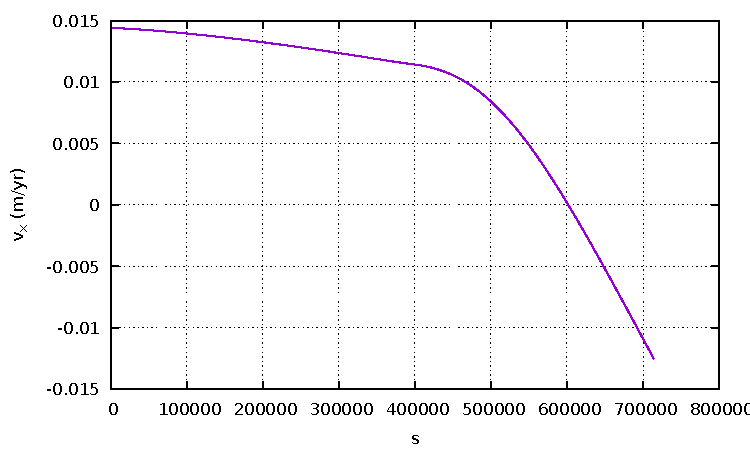
\includegraphics[width=5cm]{python_codes/fieldstone_55/images/spine_u}
%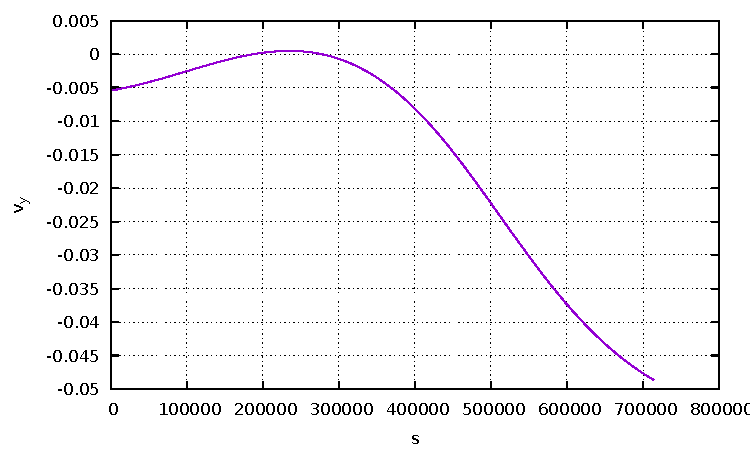
\includegraphics[width=5cm]{python_codes/fieldstone_55/images/spine_v}
%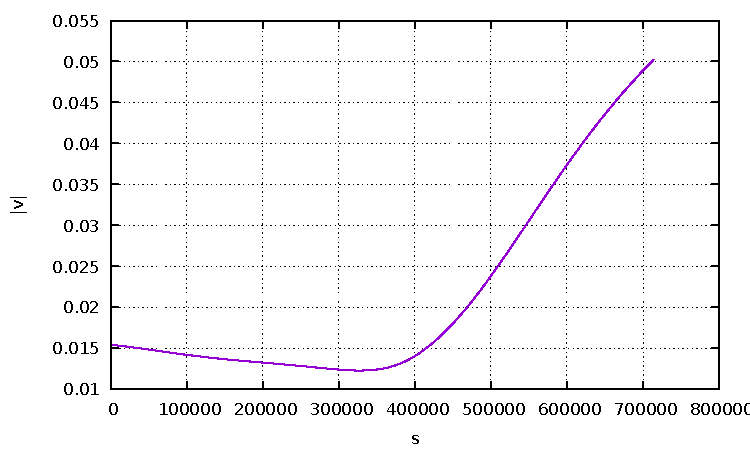
\includegraphics[width=5cm]{python_codes/fieldstone_55/images/spine_vel}\\
%{\scriptsize horizontal and vertical velocity, and velocity norm as a function 
%of $s$. $s$ is measured from 
%left to right on the midsurface and excludes the rounded edges of the slab.}
%\end{center}

We have also run this model with ASPECT for the case where free slip 
boundary conditions are prescribed on all sides. 
Velocities on the midsurface are reported hereunder alongside those
obtained with fieldstone and the BEM method.

\begin{center}
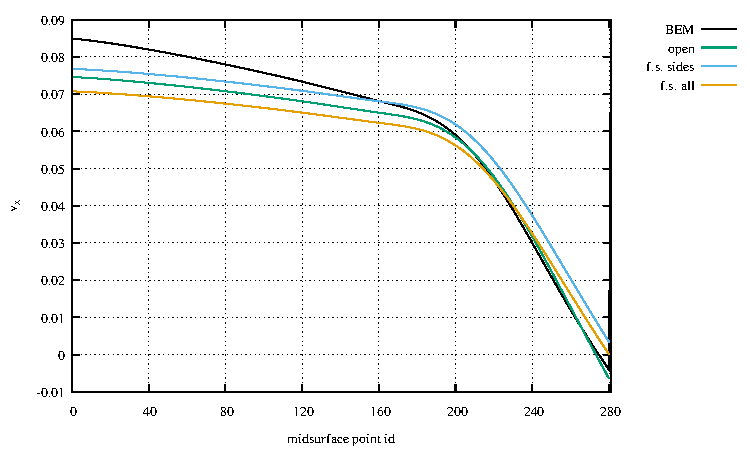
\includegraphics[width=7.5cm]{python_codes/fieldstone_55/images/u_midsurface}
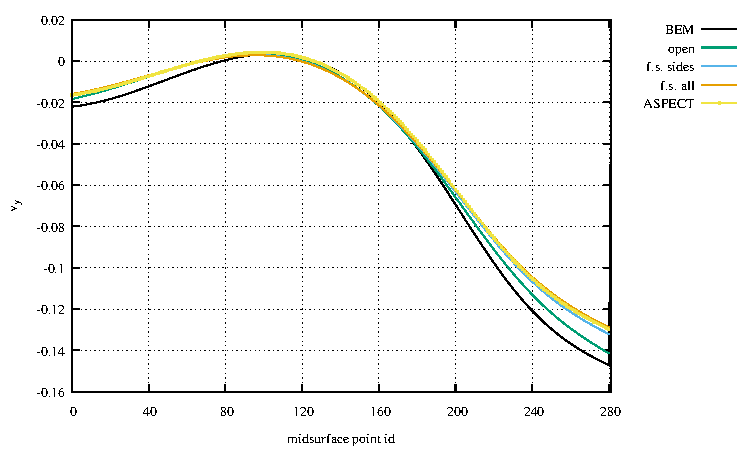
\includegraphics[width=7.5cm]{python_codes/fieldstone_55/images/v_midsurface}\\
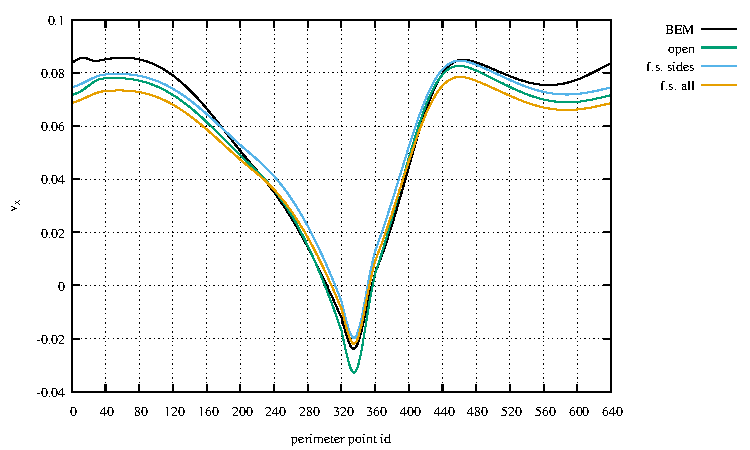
\includegraphics[width=7.5cm]{python_codes/fieldstone_55/images/u_perimeter}
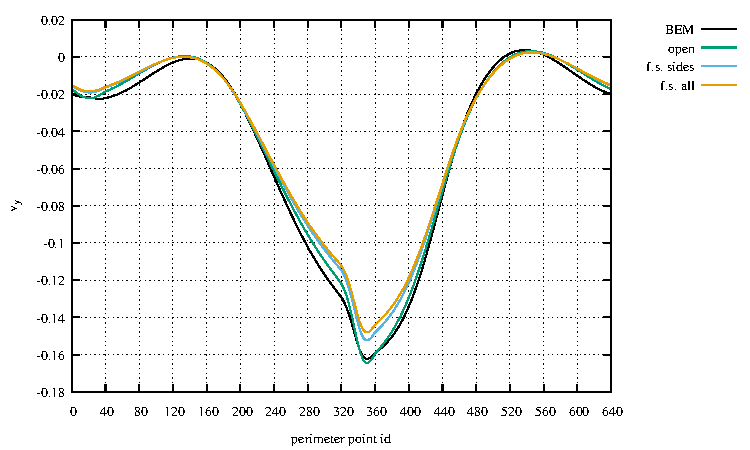
\includegraphics[width=7.5cm]{python_codes/fieldstone_55/images/v_perimeter}\\
{\captionfont Top row: midsurface velocity measurements. Bottom row: slab/plate perimeter 
velocity measurements. 'open' means no b.c. on sides and bottom; 'f.s. sides' means 
free slip b.c. on left and right sides, open at the bottom; 'f.s. all' means 
free slip b.c. on sides and bottom.}
\end{center}

\newpage
Finally, we have run this experiment over time with ASPECT (unfortunately viscosities were 100 times 
too small so that the times should be multiplied by 100):
\begin{center}
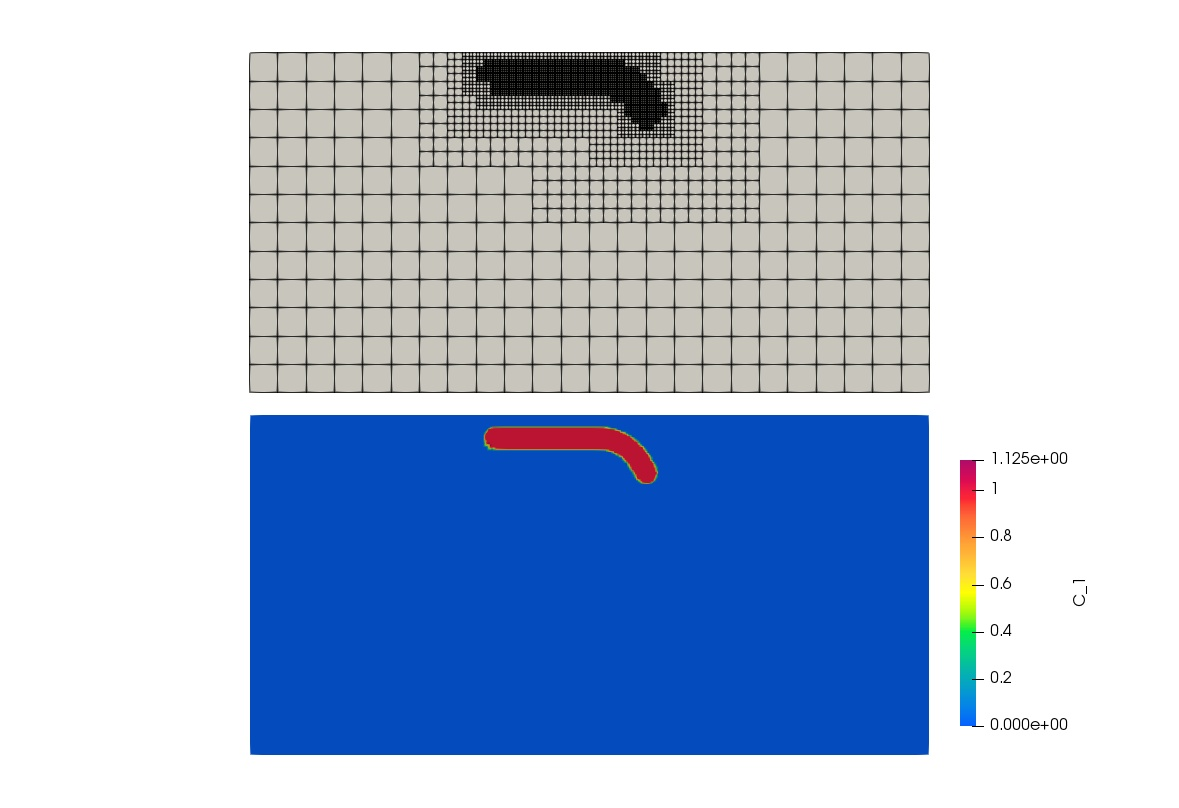
\includegraphics[width=5.26cm]{python_codes/fieldstone_55/images/aspect/grid_comp0000}
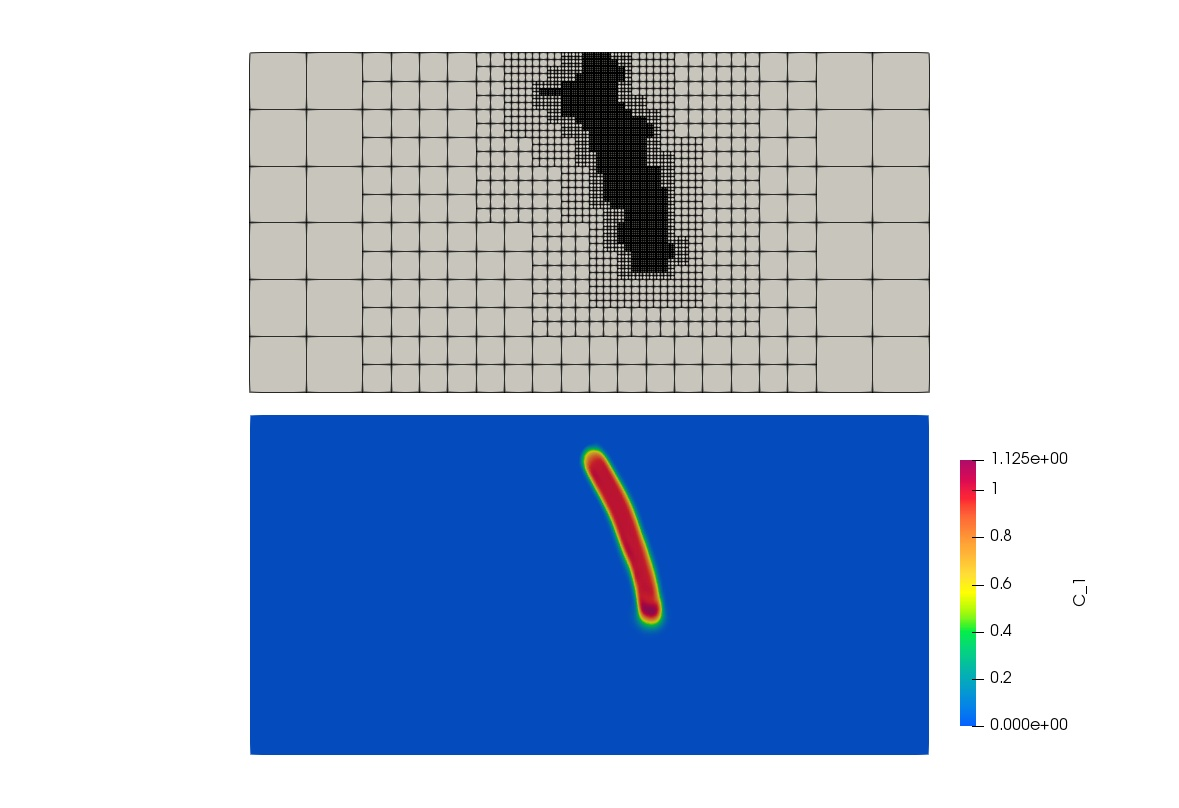
\includegraphics[width=5.26cm]{python_codes/fieldstone_55/images/aspect/grid_comp0090}
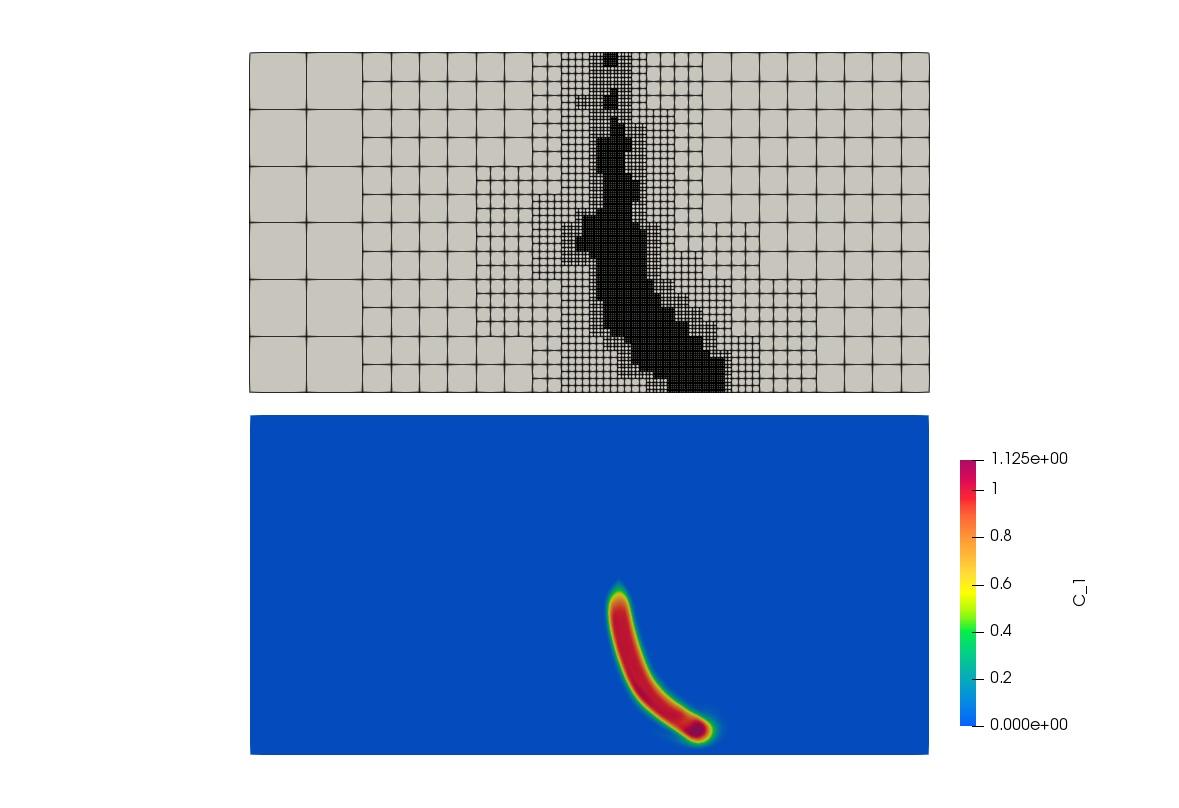
\includegraphics[width=5.26cm]{python_codes/fieldstone_55/images/aspect/grid_comp0180}\\
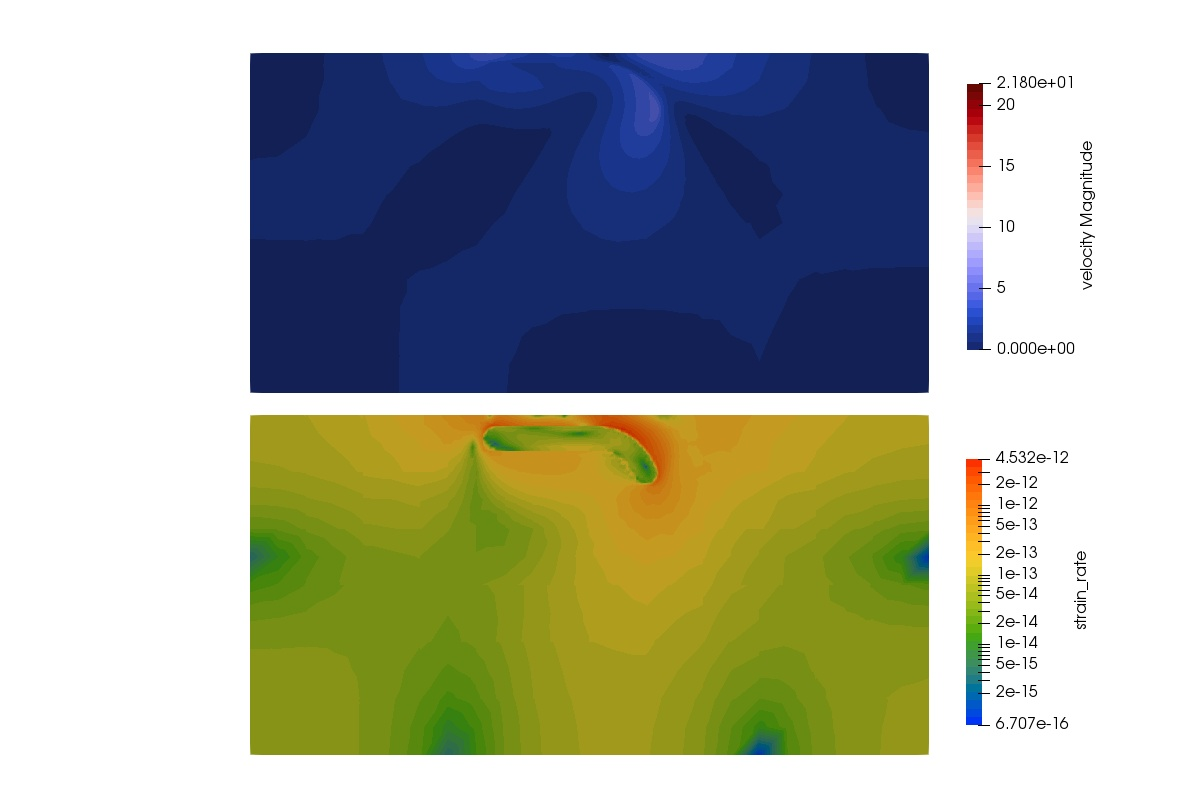
\includegraphics[width=5.26cm]{python_codes/fieldstone_55/images/aspect/vel_sr0000}
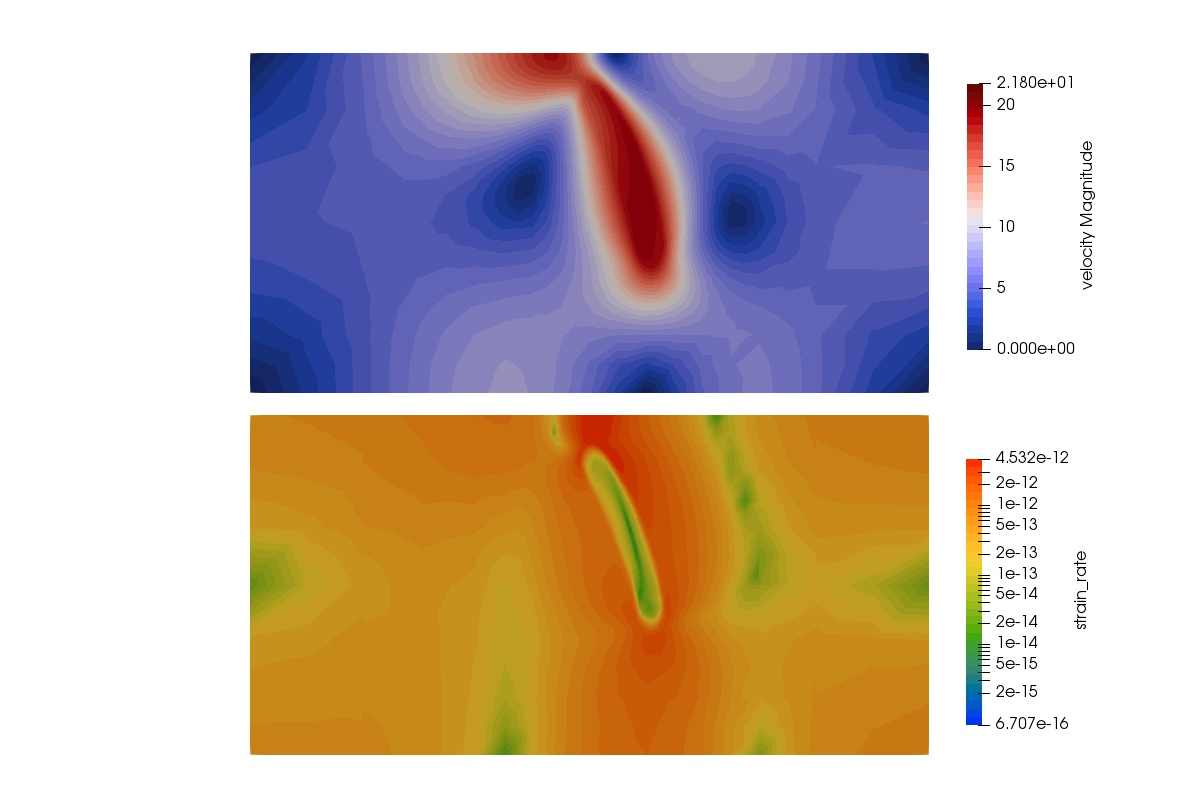
\includegraphics[width=5.26cm]{python_codes/fieldstone_55/images/aspect/vel_sr0090}
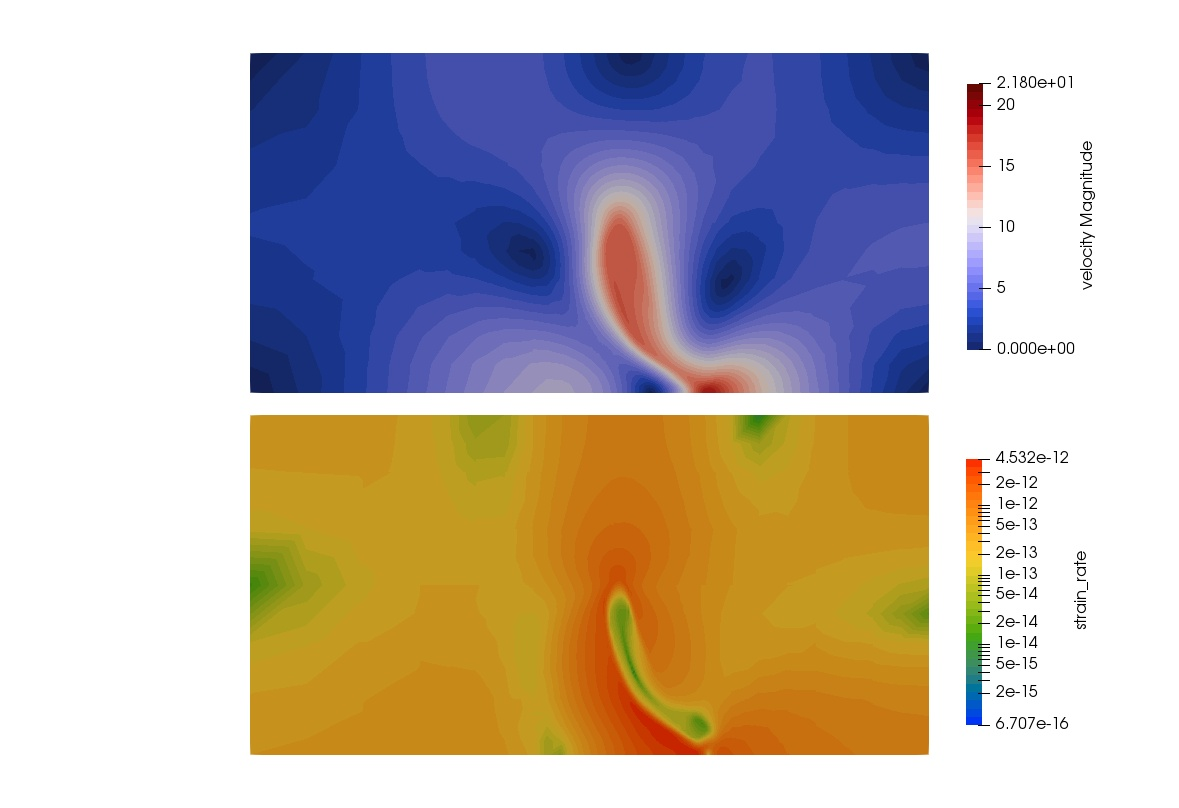
\includegraphics[width=5.26cm]{python_codes/fieldstone_55/images/aspect/vel_sr0180}\\
{\captionfont Left: t=0, middle t=64kyr, right: t=100kyr.}
\end{center}


\begin{center}
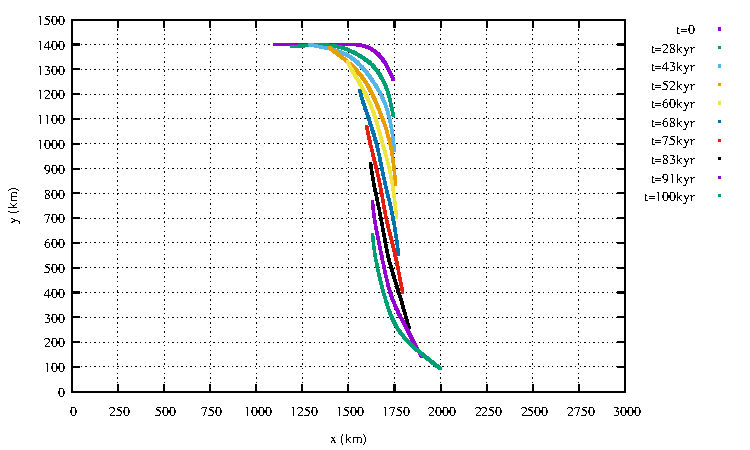
\includegraphics[width=11cm]{python_codes/fieldstone_55/images/mid_evolution}\\
{\captionfont Time evolution of the midline of the slab.}
\end{center}


\begin{center}
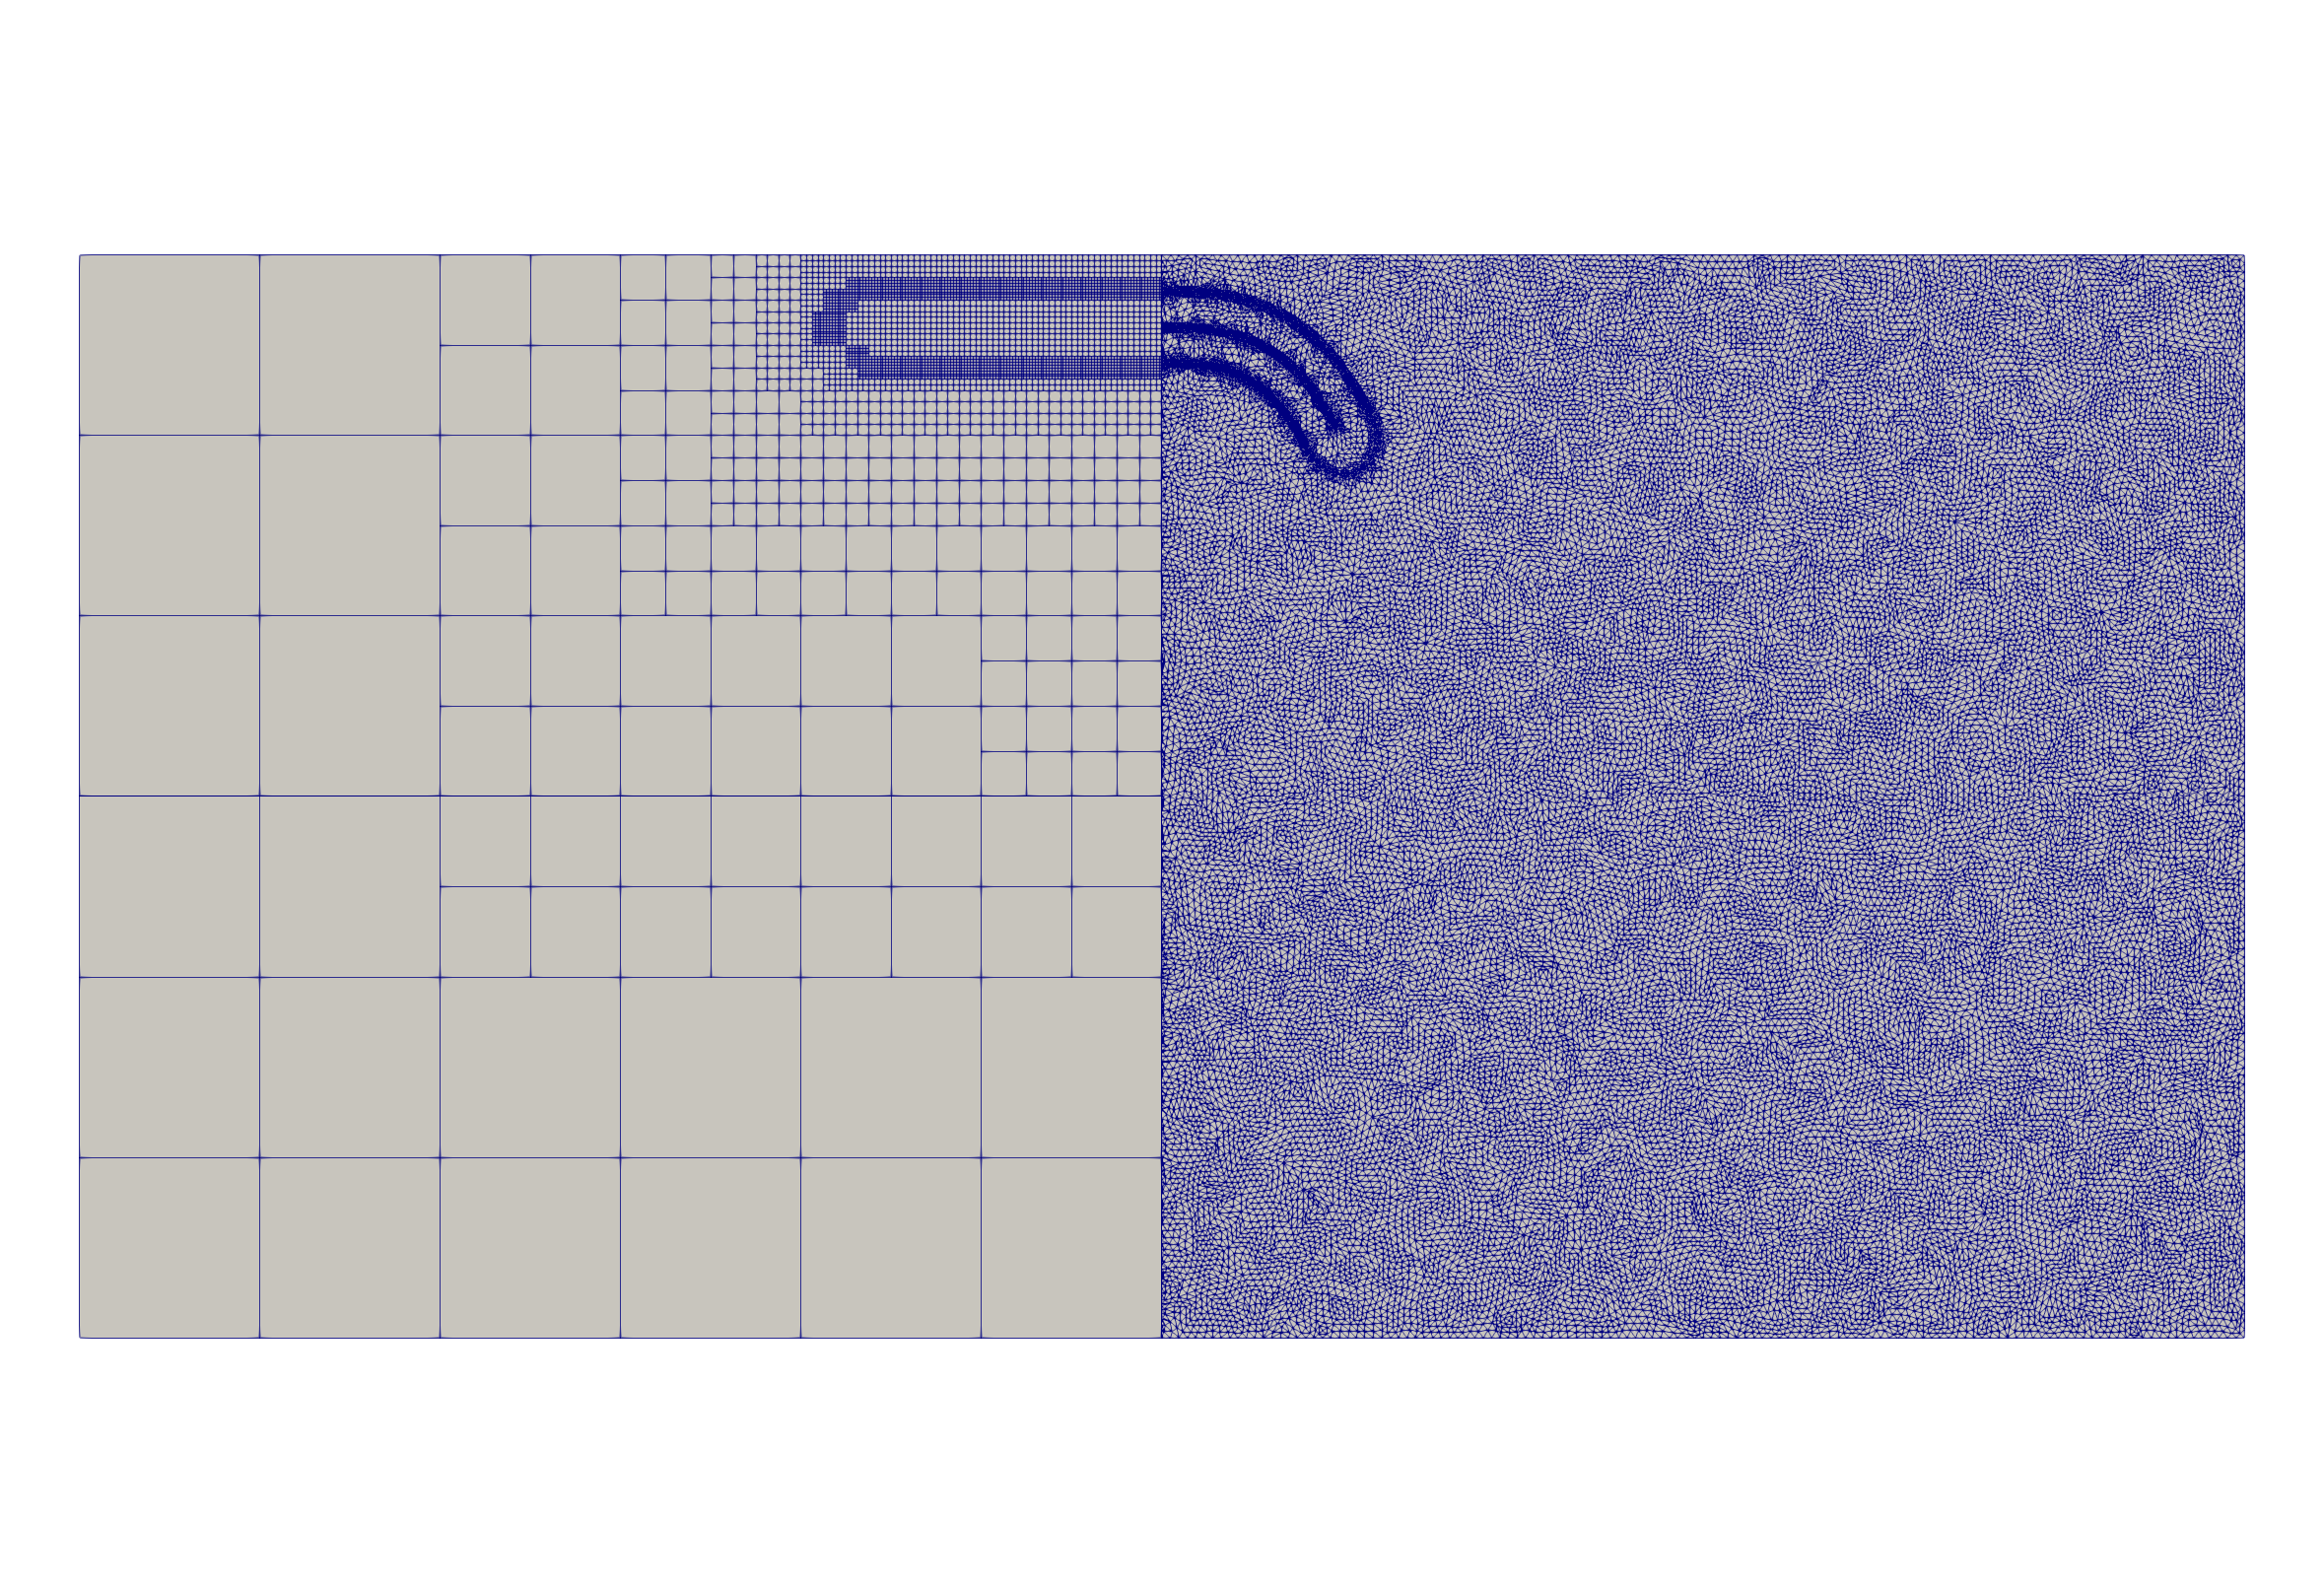
\includegraphics[width=14cm]{python_codes/fieldstone_55/images/meshes}
\end{center}

%area = 2*0.537071*h**2 + (7*h)*h , 80728764230.49994 with h=100km

\vspace{3cm}

%\begin{center}
%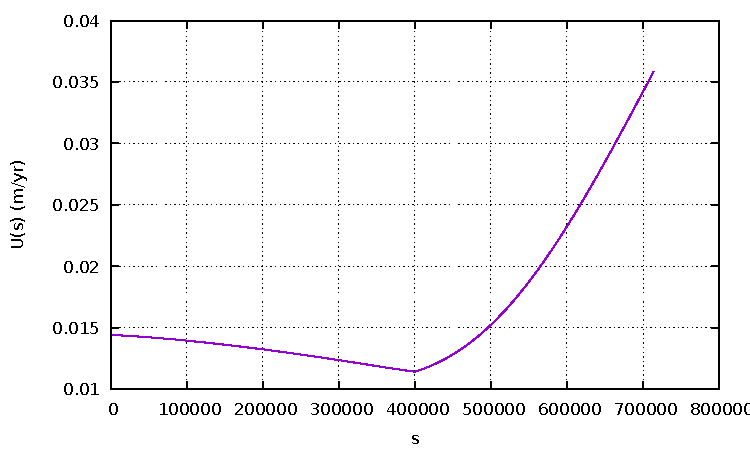
\includegraphics[width=7cm]{python_codes/fieldstone_55/images/spine_Us}
%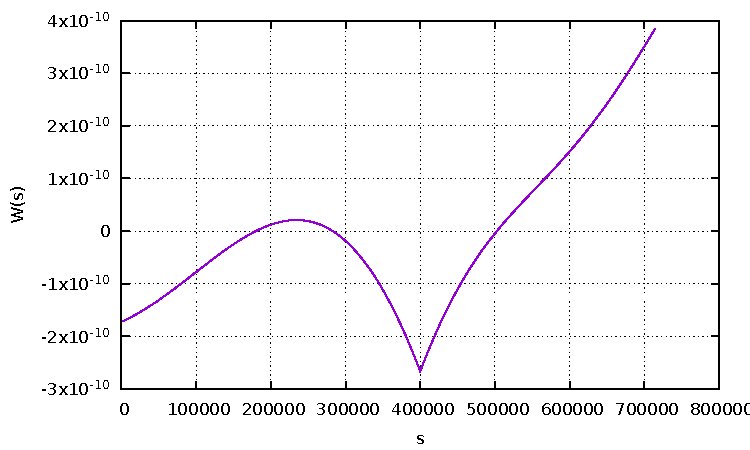
\includegraphics[width=7cm]{python_codes/fieldstone_55/images/spine_Ws}\\
%{\scriptsize Parallel and perpendicular velocity to midsurface. $s$ is measured from 
%left to right on the midsurface and excludes the rounded edges of the slab.}
%\end{center}


Literature: \cite{fogm14}
